\documentclass{exam}

\usepackage{units} 
\usepackage{graphicx}
\usepackage[fleqn]{amsmath}
\usepackage{cancel}
\usepackage{float}
\usepackage{mdwlist}
\usepackage{booktabs}
\usepackage{cancel}
\usepackage{polynom}
\usepackage{caption}
\usepackage{fullpage}
\usepackage{comment}
\usepackage{enumerate}
\usepackage{xfrac}

\newcommand{\degree}{\ensuremath{^\circ}} 
\everymath{\displaystyle}

\printanswers
\excludecomment{comment}

\ifprintanswers 
  \usepackage{2in1, lscape} 
\fi

\author{}
\date{October 2, 2013}
\title{Math 142 \\ Chapter Five Exam}

\begin{document}

  \maketitle

  \begin{questions}
    
    \question
      If $\left( \frac{2}{3}, - \frac{\sqrt{5}}{3} \right)$ is the terminal point determined by $t$, find:
      \begin{parts}
        \part[2] $\sin t$
          \begin{solution}
            $\sin t = - \frac{\sqrt{5}}{3}$
          \end{solution}

        \part[2] $\cos t$
          \begin{solution}
            $\cos t = \frac{2}{3}$
          \end{solution}

        \part[2] $\tan t$
          \begin{solution}
            $\cot t = - \frac{\sqrt{5}}{3} \cdot \frac{3}{2} = - \frac{\sqrt{5}}{2}$
          \end{solution}

        \part[2] $\csc t$
          \begin{solution}
            $\csc t = \frac{1}{\sin t} = - \frac{3}{\sqrt{5}} = - \frac{3 \sqrt{5}}{5}$
          \end{solution}

        \part[2] $\sec t$
          \begin{solution}
            $\sec t = \frac{1}{\cos t} = \frac{2}{3}$
          \end{solution}

        \part[2] $\cot t$
          \begin{solution}
            $\cot t = \frac{1}{\tan t} = - \frac{\sqrt{5}}{3}$
          \end{solution}

      \end{parts}

    \question
      If $\cot t = - \frac{1}{3}$ and $t$ is in quadrant IV

      \begin{solution}
        First find the terminal point.  Since the point is in quadrant IV, the $y$ coordinate is negative and the $x$
        coordinate is positive.

        \begin{align*}
          \frac{x}{y}  & = \frac{1}{3} \\
          y            & = 3x \\
          \\
          x^2 + y^2    & = 1 \\
          x^2 + (3x)^2 & = 1 \\
          10 x^2       & = 1 \\
          x            & = \frac{\sqrt{10}}{10} \\
          \\
          y            & = -3x \\
                       & = -\frac{3 \sqrt{10}}{10}  \\
        \end{align*}

        The terminal point is: $\left( \frac{\sqrt{10}}{10}, -\frac{3 \sqrt{10}}{10} \right)$.

      \end{solution}

      \begin{parts}
        \part[2] $\sin t$
          \begin{solution}
            $\sin t = -3 \frac{\sqrt{10}}{10}$
          \end{solution}

        \part[2] $\cos t$
          \begin{solution}
            $\cos t = \frac{\sqrt{10}}{10}$
          \end{solution}

        \part[2] $\tan t$
          \begin{solution}
            $\tan t = -3$
          \end{solution}

        \part[2] $\csc t$
          \begin{solution}
            $\csc t = - \frac{\sqrt{10}}{3}$
          \end{solution}

        \part[2] $\sec t$
          \begin{solution}
            $\sec t = \sqrt{10}$
          \end{solution}

        \part[2] $\cot t$
          \begin{solution}
            $\tan t = - \frac{1}{3}$
          \end{solution}

      \end{parts}

    \question Find the exact value of each expression.
      \begin{parts}

        \part[2] $\sin \frac{7 \pi}{6}$
          \begin{solution}
            $\sin \frac{7 \pi}{6} = - \frac{1}{2}$
          \end{solution}

        \part[2] $\cot \frac{3 \pi}{4}$
          \begin{solution}
            $\cot \frac{3 \pi}{4} = -1$
          \end{solution}

        \part[2] $\csc \frac{3 \pi}{4}$
          \begin{solution}
            $\csc \frac{8 \pi}{3} = \csc \left( \frac{2 \pi}{3} + 2 \pi \right) = \csc \frac{2 \pi}{3} = \frac{2 \sqrt{3}}{3}$
          \end{solution}

        \part[2] $\cos \frac{17 \pi}{2}$
          \begin{solution}
            $\cos \frac{17 \pi}{2} = \cos \left( \frac{\pi}{2} + 8 \pi \right) = \cos \frac{\pi}{2} = 0$
          \end{solution}

      \end{parts}

      \question[10] Express $\tan x$ in terms of $\csc x$ if the terminal point is in quadrant IV.
        \begin{solution}
          \begin{align*}
            \tan^2 x & = \frac{\sin^2 x}{\cos^2 x} \\
                     & = \frac{\sin x}{1 - \sin^2 x} \\
                     & = \frac{1}{\csc^2 x (1 - \sin^2 x)} \\
                     & = \frac{1}{\csc^2 x - 1} \\
            \tan x   & = \frac{1}{\sqrt{\csc^2 x - 1}} \\
          \end{align*}

          Tangent is negative in quadrant IV, so in quadrant IV:
          \[
            \tan x = \frac{1}{\sqrt{\csc^2 x - 1}} \\
          \]

        \end{solution}

      \question 
        \[
          f(x) = 5 \sin \left( \frac{1}{2} x - \frac{\pi}{3} \right)
        \]

        \begin{parts}
          \part[2] What is the amplitude?
            \begin{solution}
              5
            \end{solution}

          \part[2] What is the period?
            \begin{solution}
              \begin{align*}
                T = \frac{2 \pi}{\sfrac{1}{2}} = 4 \pi 
              \end{align*}
            \end{solution}

          \part[2] What is the phase shift?
            \begin{solution}
              \begin{align*}
                f(x) &= 5 \sin \left[ \frac{1}{2} \left( x - \frac{2 \pi}{3} \right) \right]
              \end{align*}

              The phase shift is $\frac{2 \pi}{3}$
            \end{solution}

          \part[5] Graph $f$
          \begin{figure}[H]
            \centering
            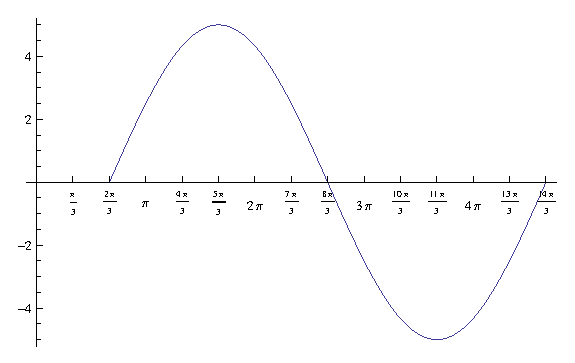
\includegraphics{graph1.eps}
            \caption{$f(x) = 5 \sin \left( \frac{1}{2} x - \frac{\pi}{3} \right)$}
          \end{figure}
        \end{parts}

  \end{questions}
\end{document}

